\documentclass[tikz]{standalone}
\usepackage{pgfplots}
\pgfplotsset{compat=1.15}
\usepackage{mathrsfs}
\usetikzlibrary{arrows,calc}
\usepackage{tkz-euclide}

\usepackage{fp}
\pagestyle{empty}

\definecolor{AngleClr}{rgb}{0,0.39215686274509803,0}
\definecolor{ShapeClr}{rgb}{0.6,0.2,0}

\begin{document}

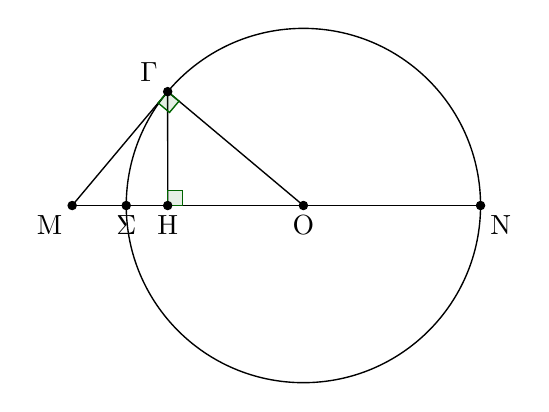
\begin{tikzpicture}[scale=.75]
\tkzSetUpLine[line width=1pt,color=black]
\tkzSetUpPoint[fill=black]

\tkzDefPoints{0/0/O,3/0/N,-3/-0.4/E,-3/0/X}

\tkzDefPoint(140:3){A}

\tkzDefPointsBy[projection=onto N--X](A){H}


\tkzDrawCircle[color=black,fill=white,line width=0.5pt](O,X)

\tkzDrawSegments[line width=0.5pt,color=black](O,A)


\tkzDefLine[tangent at=A](O) \tkzGetPoint{h}

\tkzInterLL(A,h)(N,X) \tkzGetPoint{M}

\tkzDrawSegments[line width=0.5pt,color=black](M,N A,H A,M)


\tkzMarkRightAngle[line width=0.5pt, size=.25,color=AngleClr,fill=AngleClr,fill opacity=0.1](O,A,h)

\tkzMarkRightAngle[line width=0.5pt, size=.25,color=AngleClr,fill=AngleClr,fill opacity=0.1](A,H,O)

\tkzDrawPoints[size=3](A,O,M,N,X,H)
\tkzLabelPoint[above left](A){$\rm \Gamma$}
\tkzLabelPoint[below](O){$\rm O$}

\tkzLabelPoint[below left](M){$\rm M$}
\tkzLabelPoint[below right](N){$\rm N$}
\tkzLabelPoint[below](X){$\rm \Sigma$}
\tkzLabelPoint[below](H){$\rm H$}

\end{tikzpicture}
\end{document}
